\documentclass[11pt]{article}
\usepackage{amsmath,amsfonts,amssymb}
\usepackage{hyperref}
\hypersetup{
	colorlinks=true,
	linkcolor=blue,
	urlcolor=cyan
	}
\usepackage[margin=1in]{geometry}
\usepackage{graphicx}
\usepackage[dvipsnames]{xcolor}
\newcommand{\red}{\color{red}}
\newcommand{\black}{\color{black}}
\newcommand{\blue}{\color{MidnightBlue}}
\newcommand{\jean}[1]{{\color{blue} [Jean: #1]}}


\setlength{\parindent}{0pc}
\setlength{\parskip}{10pt}

\title{STAT157 HW 8}
\date{March 8, 2023}

\begin{document}

\maketitle

\hfill \textbf{Due Wednesday, March 15 at 11:59pm}

\section*{Deliberate Practice: Invalidating Considerations}

\emph{Expected completion time: 120 minutes}

This exercise follows the activity in last week's discussion.
We will use the following simplified model for invalidating considerations:
\begin{itemize}
	\item Suppose you want an 80\% confidence interval around some quantity
	\item You have an initial distribution $p_0$ for what happens in a “normal” world. For example, maybe this is the distribution that you get by looking at a reference class.
	\item After brainstorming invalidating considerations, you realize that there is a small probability $\epsilon$ that you are instead in a “crazy” world, in which case your distribution is instead $p_1$.
	\item Your new probability distribution is therefore the mixture $(1 - \epsilon) p_0 + \epsilon p_1$.
\end{itemize}

For each of the following examples of $p_0$, $p_1$, and $\epsilon$, do the following:
\begin{itemize}
	\item Give an 80\% confidence interval when accounting for the $\epsilon$ probability of a ``crazy'' world. Your interval should be centered, i.e.~your lower and upper bounds should be the 10th and 90th percentiles of the mixture distribution.
	\item Confirm your reasoning by simulation: using Python, draw 1000 samples from $(1 - \epsilon) p_0 + \epsilon p_1$, and use them to estimate the 10th and 90th percentiles of this distribution. Sampling from a mixture happens in two steps:
		\begin{itemize}
			\item Sample from a Bernoulli($\epsilon$) to choose between $p_0$ and $p_1$.
			\item Sample from the chosen distribution (in this exercise the distributions will be uniform).
		\end{itemize}
\end{itemize}

\newpage

\begin{enumerate}
	\item Non-overlapping uniform distributions 
	\begin{itemize}
		\item $p_0 = \text{Uniform}(0, 2)$
		\item $p_1 = \text{Uniform}(2.5, 3)$
		\item (a) $\epsilon = 0.05$, (b) $\epsilon = 0.1$, (c) $\epsilon = 0.2$
	\end{itemize}

\begin{center}
	\begin{figure}[h!]
	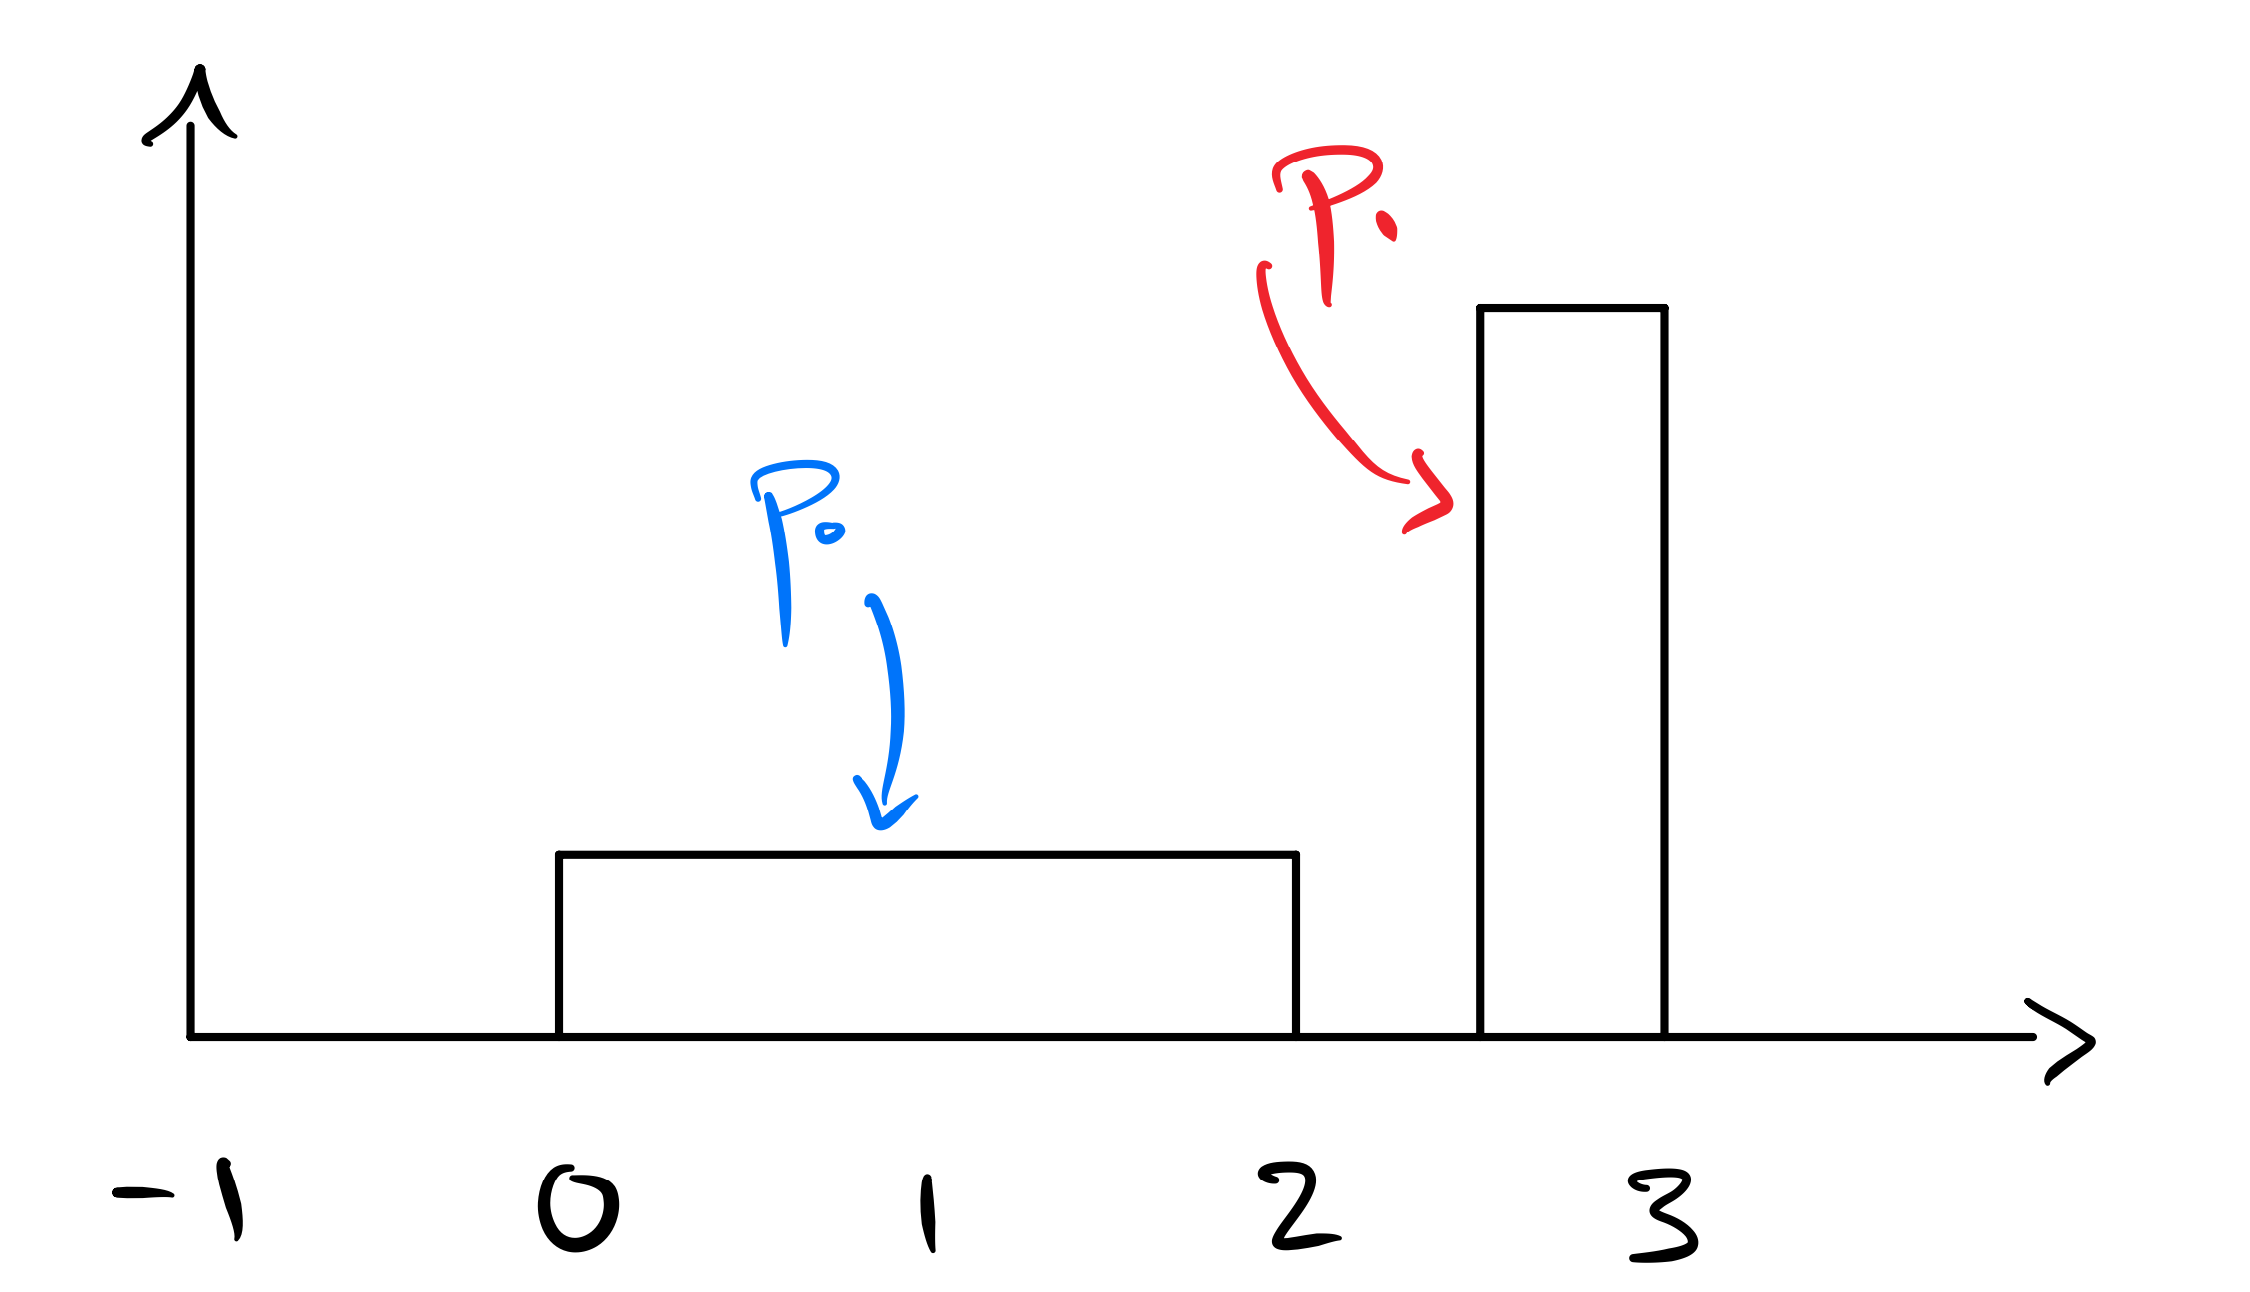
\includegraphics[width=260pt]{non-over.png}
	\caption{Non-overlapping uniform distributions}
	\end{figure}
\end{center}


\item Overlapping uniform distributions
	\begin{itemize}
		\item $p_0 = \text{Uniform}(0, 2)$
		\item $p_1 = \text{Uniform}(1, 3)$
		\item (a) $\epsilon = 0.05$, (b) $\epsilon = 0.1$, (c) $\epsilon = 0.2$
	\end{itemize}

\begin{center}
	\begin{figure}[h!]
	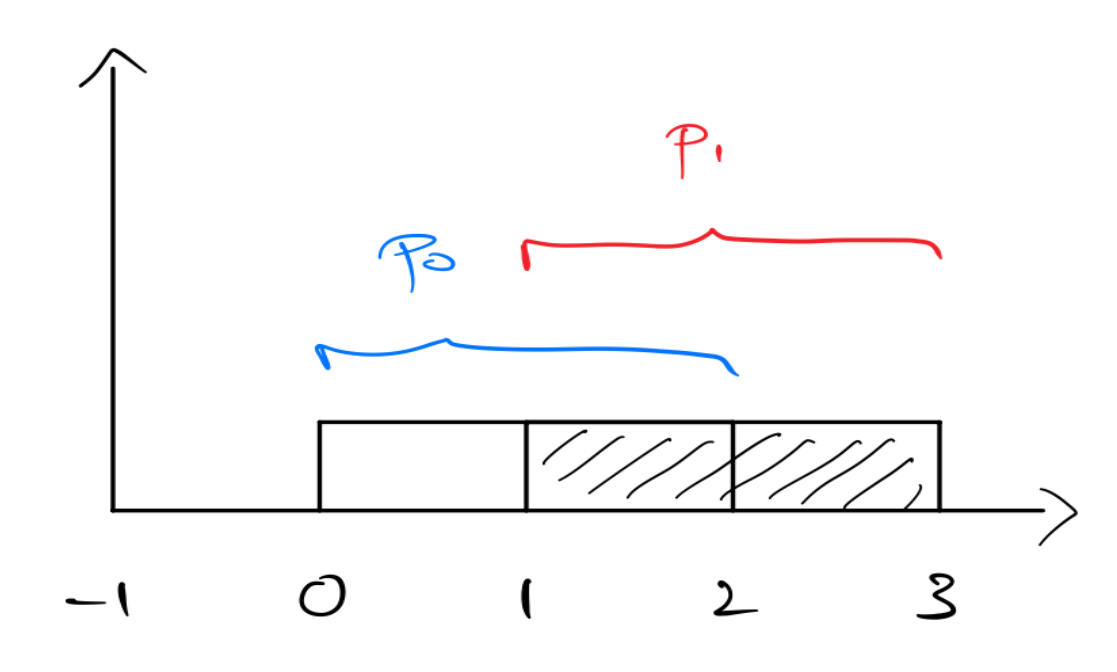
\includegraphics[width=260pt]{1.png}
	\caption{Overlapping uniform distributions}
	\end{figure}
\end{center}

% \item Point masses on both sides 
% 	\begin{itemize}
% 		\item $p_0 = \text{Uniform}(1,2)$ 
% 		\item $p_1 = 0.5 \text{Dirac}(0) + 0.5 \text{Dirac}(3)$
% 		\item (a) $\epsilon = 0.05$, (b) $\epsilon = 0.1$, (c) $\epsilon = 0.2$
% 	\end{itemize}

% \begin{center}
% 	\begin{figure}[h!]
% 	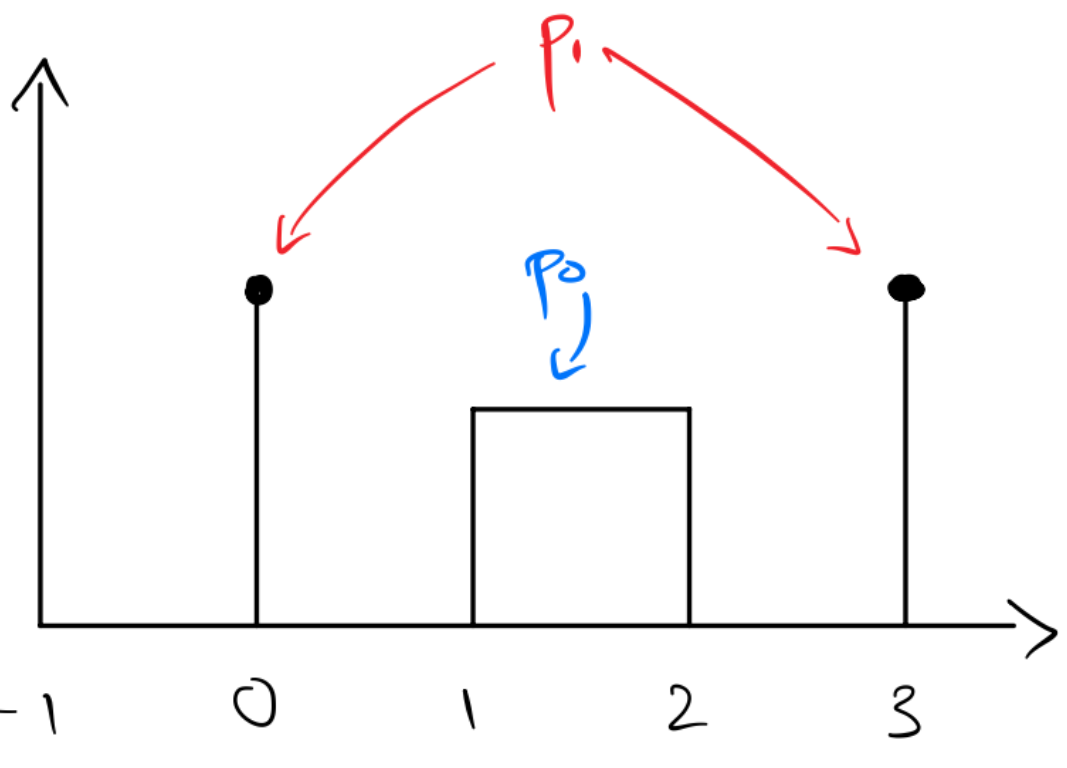
\includegraphics[width=240pt]{3.png}
% 	\caption{Point masses on both sides}
% 	\end{figure}
% \end{center}


% \item Tetris blocks
% 	\begin{itemize}
% 		\item $p_0$ has pdf $f(x) = 0.5$ if $0 \leq x < 1$, $f(x) = 1$ if $1 \leq x < 1.5$, and $f(x) = 0$ otherwise
% 	\item $p_1 = \text{Uniform}(2.5, 3)$
% 		\item (a) $\epsilon = 0.05$, (b) $\epsilon = 0.1$, (c) $\epsilon = 0.2$
% 	\end{itemize}

% \begin{center}
% 	\begin{figure}[h!]
% 	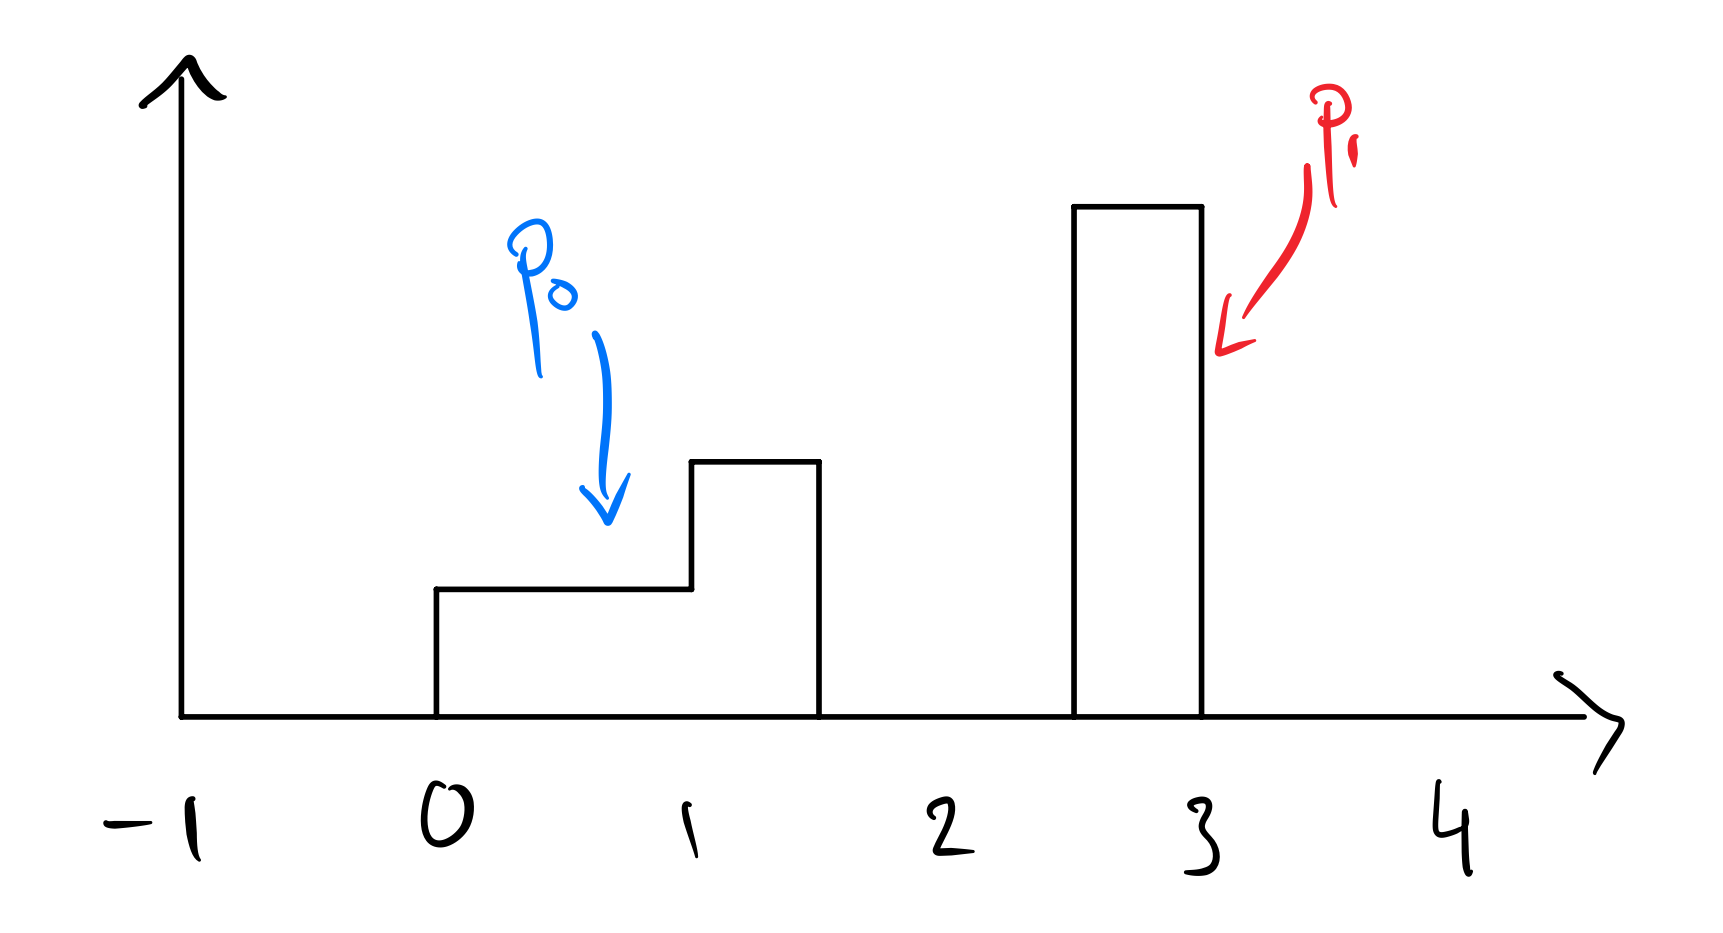
\includegraphics[width=260pt]{4.png}
% 	\caption{Tetris blocks}
% 	\end{figure}
% \end{center}

\end{enumerate}

On Gradescope, please also submit the time it took to complete this exercise.

\newpage

\section*{Deliberate Practice: Numerical Sensitivity}

\emph{Expected completion time: 180 minutes}

Consider the formula for the number of days $T$ until the peak of Omicron that we used in the \emph{Turning Considerations into Probabilities} lecture:
$$T = \log_2(N / 2 N_0) \cdot t + \Delta_0 + \Delta_1,$$
where:
\begin{itemize}
	\item $N$ is the total number of future UK Omicron cases
	\item $N_0$ is the current number of UK Omicron cases
	\item $t$ is the Omicron doubling time
	\item $\Delta_0$ is the lag between case peak and hospital peak
	\item $\Delta_1$ is the lag between single-day hospital peak and 7-day average hospital peak
\end{itemize}

Using simulations, we will assess the sensitivity of this formula to variations of its five inputs.

\begin{enumerate}
	\item Suppose the inputs are sampled independently from Normal and LogNormal distributions. For this, sample $\alpha, \beta, \gamma$, and $\delta$ independently from Normal(0, 1), and define the inputs $N$, $N_0$, $t$, and $\Delta$ as follows:
	\begin{itemize}
		\item $N = \exp(15.57 + 0.30 \cdot \alpha)$ 
			\begin{itemize}
				\item This \href{https://www.johndcook.com/blog/2022/02/24/find-log-normal-parameters/}{means} that $N$ follows a LogNormal distribution with mean $6.7 \times 10^6$ and standard deviation $4 \times 10^6$.
			\end{itemize}
		\item $N_0 = \exp(12.18 + 0.06 \cdot \beta)$
			\begin{itemize}
				\item This \href{https://www.johndcook.com/blog/2022/02/24/find-log-normal-parameters/}{means} that $N_0$ follows a LogNormal distribution with mean $0.2 \times 10^6$ and standard deviation $0.05 \times 10^6$.
			\end{itemize}
		\item $t = 2.4 + 0.5 \cdot \gamma$
		\item $\Delta = \Delta_0 + \Delta_1 = 12 + 3 \cdot \delta$.
	\end{itemize}
	Sample the inputs in this way 1000 times, computing each time the corresponding value of $T$ using the formula above. Plot the histogram of the distribution of $T$: what are its 10th, 25th, 50th, 75th, and 90th percentiles?
	\item Increase the standard deviation of $N$ while leaving the other distributions constant: for this, sample $\alpha$ from Normal(0, 4) rather than Normal(0, 1). Do the same but for $\Delta$ instead: double the standard deviation of $\delta$, while leaving the other distributions constant. Which of these leads to the greatest increase in the variance of $T$?
	\item Replace the Normal distributions by Student's $t$ distributions: instead of sampling $\alpha$, $\beta$, $\gamma$ and $\delta$ from Normal(0, 1), sample them from Student($\nu$ = 5). Plot the histogram of the distribution of $T$: how did using a $t$ distribution instead of a Normal change the quantiles and variance of $T$? 
	\item Repeat your simulation with $\nu = 3$, $\nu = 7$ and $\nu = 9$: how does the degrees of freedom parameter $\nu$ affect the distance between the 10th and 90th percentiles of $T$?
	\item Suppose now that instead of being independent, the inputs are correlated. That is, sample $[\alpha, \beta, \gamma, \delta]^\top$ from a multivariate Gaussian distribution: 
		$$
		\begin{bmatrix}
			\alpha\\
			\beta\\
			\gamma\\
			\delta	
		\end{bmatrix} \sim \text{Normal}(\mathbf{0}, \mathbf{\Sigma}),
		\text{ with }
		\mathbf{\Sigma} = \begin{bmatrix}
				1 & \rho & \rho & \rho\\
				\rho & 1 & \rho & \rho\\
				\rho & \rho & 1 & \rho\\
				\rho & \rho & \rho & 1
			\end{bmatrix},
		\text{ and } \rho \in \left(-\frac 1 3, \frac 1 3\right).
		$$
	Draw 1000 samples, and plot a histogram of the values of $T$. Do the 10th and 90th quantiles get closer together or farther apart as the correlation parameter $\rho$ increases from 0 to $\frac 1 3$? as $\rho$ decreases from 0 to $- \frac 1 3$?
\end{enumerate}


On Gradescope, please also submit the time it took to complete this exercise.

\section*{Predictions}

\emph{Expected completion time: 120 minutes} 

Register the following predictions. You can submit them by going to \href{https://docs.google.com/forms/d/1zfza4lPpQWRJDRBghY6a9-HK3erBo32wJBQy-BGfhBA/edit}{this URL} and following the form's instructions. For these predictions, (and all predictions about the future throughout this class), we encourage you to use external sources -- by googling things, reading news articles, talking to friends who follow politics or music stats, etc.

\begin{enumerate}
	\item Will the Montreal REM line between Brossard and Central Station open to the public before May 10th, 2023? This question will resolve based on whether \href{https://en.wikipedia.org/wiki/Brossard_station}{the wikipedia article for Brossard station} mentions that the station has opened. The wikipedia article should also cite an article that shows that the station has indeed opened.
	\item How many NYT headlines/ledes in the \href{https://www.nytimes.com/section/nyregion}{New York section} dated between Mar 16 and Mar 23 (included) will include Eric Adams' name? 
	\item Will \href{https://leginfo.legislature.ca.gov/faces/billNavClient.xhtml?bill_id=202320240AB1700}{California Assembly Bill 1700} pass the California Assembly by May 10th, 2023?
\end{enumerate}

For each question, submit an inclusive 80\% confidence interval or your probabilities, as well as an explanation of your reasoning (1-2 paragraphs). \textbf{Please include a copy of your google form responses with your Gradescope submission.} On Gradescope, please also submit the time it took to complete this exercise.

\end{document}
